\chapter{\textit{Grasp}について}
\label{graspについて}

\section{概要}
\ref{related_works}章では、FelsのEmbodimentを説明し、「身体化するまでの過程」から本研究の位置付けを整理し、先行研究や作品実践に対しても同じ視点から相違点の説明を試みた。
本章では、「身体化するまでの過程」について\textit{grasp}という概念を定義し、Felsの議論との関係性と、この概念に到達するまでのプロトタイピングから概念の妥当性を補強する。\\

\section{\textit{grasp}の定義}
本研究での\textit{grasp}とは、\textbf{「人がある対象に注意や目的意識を抱き、注意を向けた対象を確かめるため、または目的の達成に向けて試行を行う期間」}と定義する。
例えば、楽器の習得過程において、弾きこなしたいフレーズを定め、それを達成するまでに試行錯誤をし、達成できるようになるまでの期間を指す。また、そのように熟達していくと、熟達をきっかけとして別の目標が芽生える。当初目指していた、あるいはやってみる前から想起できていたこととは異なることについて目的意識が芽生える。\\
これは\textit{grasp}の過程における重要な性質の1つであると考えている。

\section{Felsの議論との関係性}
このコンセプトについて、FelsのEmbodimentのカテゴリとの関係性を明確にする。\\
\textit{grasp}は、FelsのResponseやControl、そしてBelongingが達成されるまでの過程を捉える期間である。\\

\section{\textit{grasp}に辿り着くまでのプロトタイピング}
\label{prototyping_concept_making}
作品のもととなった試行は当初、「動きのスケッチツール」というまったく別の目的で作られたシステムである。\\
ピアノを弾く時のように、人は10本ある指を同時に操り、その組み合わせから柔軟で緻密な動作を作ることができる。手のストロークを記録し、静止画をスケッチする場として「紙とペン」があるように、手の動きをそのまま記録し、「動きをスケッチする」場として新しいインターフェースを設計することを案じていた。\\
しかし手指は人間の身体の中でもとりわけ随意に動かすことのできる器官である。だからこそ、動きを入力するためのインターフェースは、手と異なる形状であったとしても自在に操ることができるのではないか。もしそうであるならば、人間の身体構造による制約を超えた「動きのスケッチ」が達成できる、と考えた。\\
そうして、手指の動きをトラッキングしつつ、画面上でその動きは別の形へマッピングされて動くインターフェースを制作し、IAMAS Open House 2022にて展示した。この時点では、動きを記録する機能は存在しておらず、あくまで手と、それに伴って動く手指とは異なる形の動きが確認できるだけのものであった。\\

\begin{figure}[H]
  \centering
  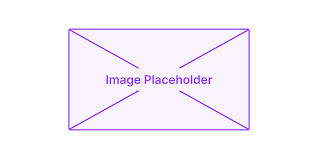
\includegraphics[width=15cm]{img/placeholder.png}
  \caption{IAMAS Open House 2022での展示のようす(2022年)}
  \label{fig:exhibit_2022}
\end{figure}

しかし実際に展示を行うと、「身体の変換」を扱った表現については、当初想定していなかった仕方で受容されることがわかった。まず1つ目に、構造としては単に手の指の動きが、別の構造にマッピングされただけであるのに、別の構造の手を動かす感覚はそれだけで「快」がある体験だということである。その「快」の正体はこの時点ではわからなかったが、手指の変換が3パターン展示された状態のこの展示で、10分以上興味を持って体験する方が複数名いた。またもう1つに、制作されたプロトタイプを展示した際、指先を動かすだけでなく、カメラに対して手を近づけたり遠ざけたり、手を裏返したりするなど、さまざまな体験の方法が現れたことに興味を持った。これは、手指の動きが別の形状にマッピングされたことで、「反応している」ということは分かっていても「どのように反応しているのか」についてははっきりせず、それを確かめるように身体を動かしているのだと考えた。変換方法を実装した制作者は仕組みを知ってしまっているので、こうした試行は起こり得ないが、どのように変換されているのかを知り得ない体験者は、自身の体を動かして観察されたことでのみ、その動作原理を推測することになるので、最初にどう身体を動かしたかによって、動作原理をどう認識するかに違いが現れるのではないかと考えた。これをきっかけとして、手指の運動を用いた表現について「動きのスケッチツール」というテーマから離れ、「手指の変換表現」について幅広く検討する中で、こうした興味を掘り下げていくことにした。

「快」の正体に迫る上で、仮説として「手指特有の動きに対する美的関心(動きに対する快)」、「手指を動かすことに対する快(身体動作における快)」が挙げられる。\\
そこで、インタラクションのあるものについての発散と、インタラクションのないモーショングラフィックについての発散を行なった。それを踏まえて、インタラクションのあるものについての発散を試みた。


\section{\textit{grasp}の性質}
\textit{grasp}には二つの性質がある。一つは、時間幅が注意を向けている対象によって、長い場合と短い場合があることである。目的意識が芽生えてからスムーズに操作できるようになる場合、'reach'から'manipulate'が近く、\textit{grasp}は短い、すなわち直感的で使いやすいものとして経験される。その一方、目的意識が芽生えてから試行錯誤を伴い、習熟に長い期間を要する場合、\textit{grasp}は長く、もどかしさを経験し、操れるようになった時に達成感を経験する。\\

二つ目に、\textit{grasp}の過程で他のことに対する意識が次々と芽生えることがある。具体的には「やってみるまでわからない」といった経験や、物事に対する解像度が高まる中で、当初とは異なる意識が芽生える状況に相当する。\\

このコンセプトを展開し、「試行錯誤の余地」を設計することを目指したのが、修士作品《Grasp(er)》である。この作品では、\textit{grasp}を経験する中で、個人による創造的な活動が生まれ、\textit{grasp}という動作を行っているのではなく、そこに'er'の接尾辞がついた'Grasper'であると名付けた。